%
% $RCSfile: information_science.tex,v $
%
% Copyright (C) 2002-2008. Christian Heller.
%
% Permission is granted to copy, distribute and/or modify this document
% under the terms of the GNU Free Documentation License, Version 1.1 or
% any later version published by the Free Software Foundation; with no
% Invariant Sections, with no Front-Cover Texts and with no Back-Cover
% Texts. A copy of the license is included in the section entitled
% "GNU Free Documentation License".
%
% http://www.cybop.net
% - Cybernetics Oriented Programming -
%
% http://www.resmedicinae.org
% - Information in Medicine -
%
% Version: $Revision: 1.1 $ $Date: 2008-08-19 20:41:07 $ $Author: christian $
% Authors: Christian Heller <christian.heller@tuxtax.de>
%

\section{Information Science}
\label{information_science_heading}
\index{Information Science}
\index{Scientific Inventions}
\index{Robot}
\index{Computer}
\index{Hardware}
\index{Software}
\index{Informatics}
\index{Abstract Model}

\emph{Science} is one form in which humans express their aspiration for
\emph{Perception}. It should -- but unfortunately not always does -- serve the
well-being of people. Similarly, scientific \emph{Inventions} usually are to
ease human's life.

\begin{figure}[ht]
    \begin{center}
        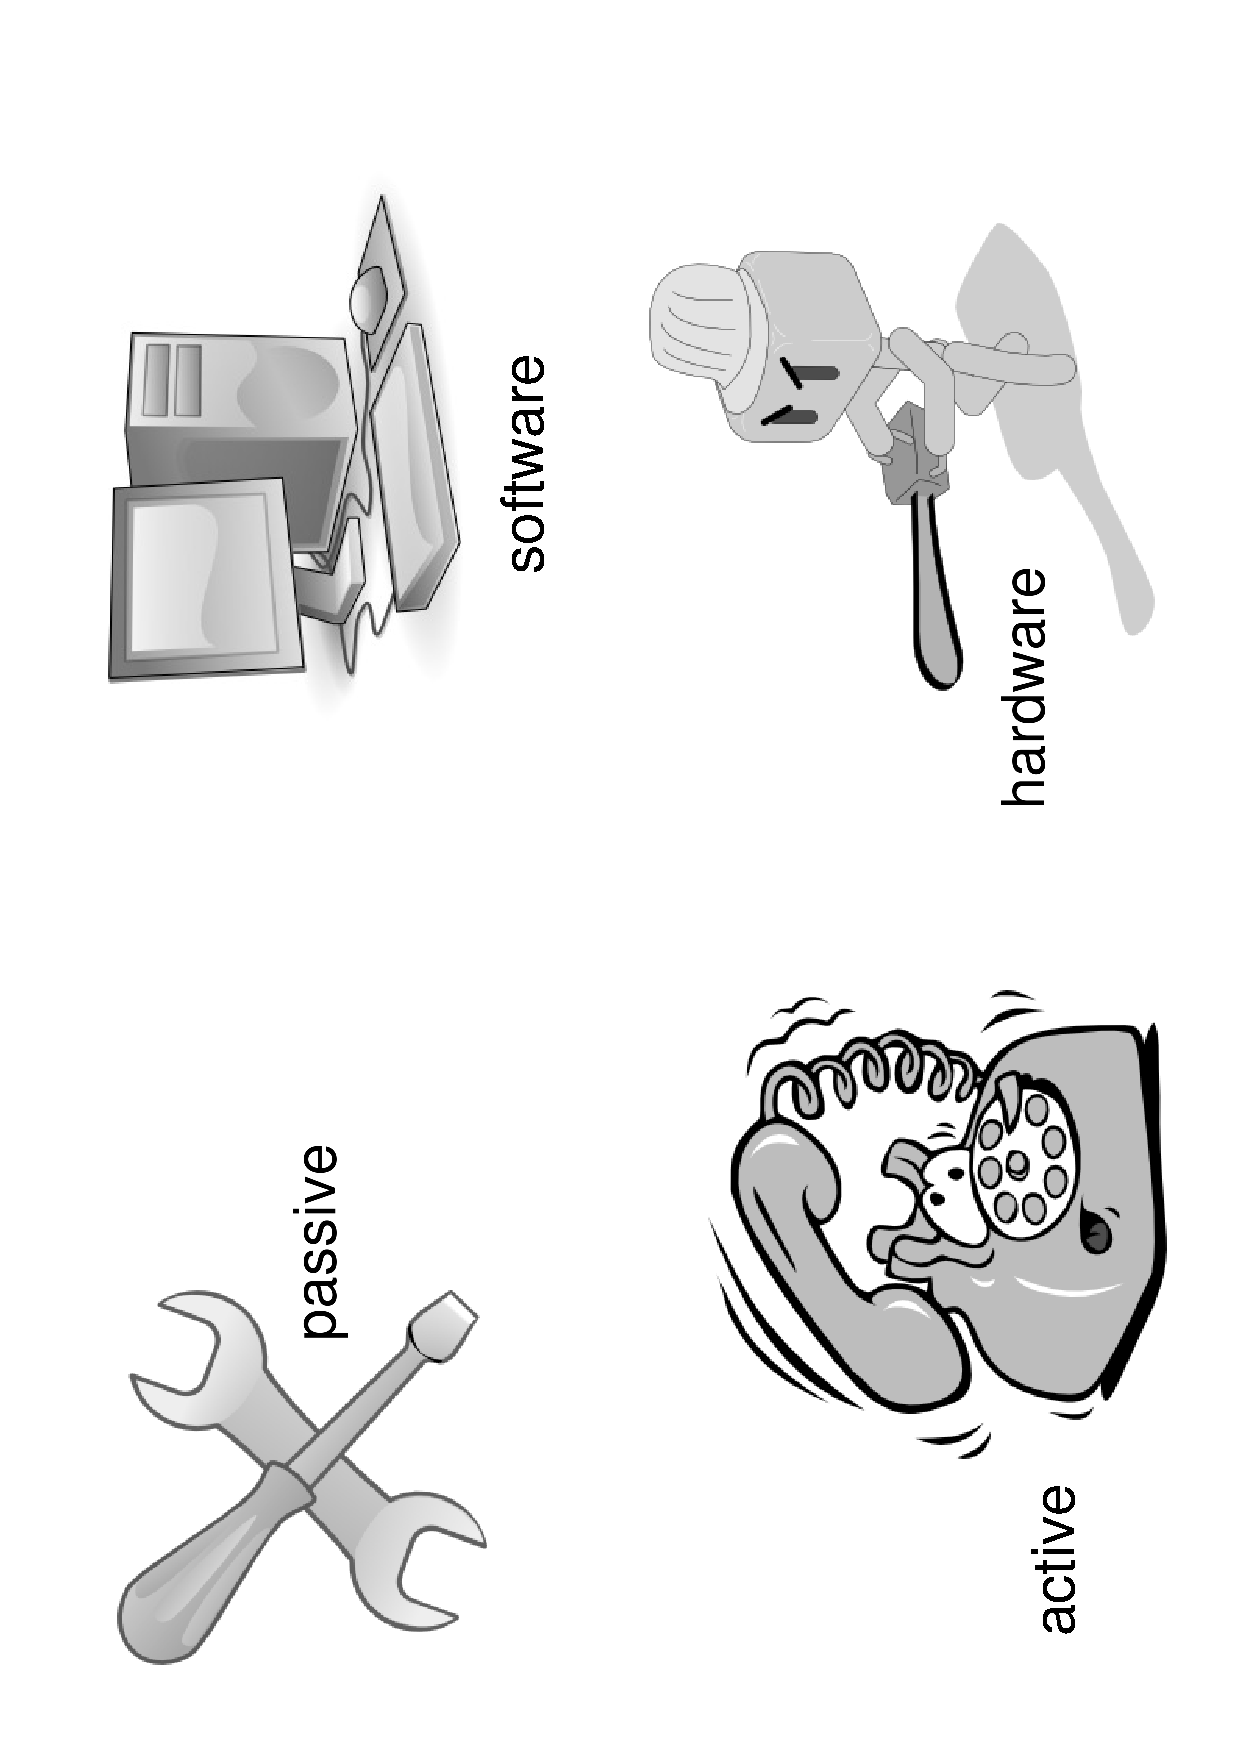
\includegraphics[scale=0.3,angle=-90]{graphic/inventions.pdf}
        \caption{Scientific Inventions}
        \label{inventions_figure}
    \end{center}
\end{figure}

The results of many technical inventions are \emph{Tools}, \emph{Machines} or
\emph{Robots} (figure \ref{inventions_figure}). A passive tool is a mostly
simple device used by humans to carry out a task better. The word machine is
used to describe advanced, active tools which can run by themselves, only
driven by an external force like steam or electrical energy. A robot, finally,
is an enhanced machine which may imitate human behaviour (humanoid) or take
over (industrial) tasks that are too dirty, dangerous, difficult, repetitive or
dull for humans \cite{wikipedia}. Its parts are often called \emph{Hardware}.
It does not necessarily have the same shape as the human body but can come very
close. Also, it contains some pieces of rudimentary \emph{Intelligence} that
lets it act alone (autonomous). The intelligence basically controls the way in
which the robot functions what is sometimes called \emph{Workflow} or
\emph{Program}. That must be encoded, for example in form of a \emph{Punchcard}
or pieces of \emph{Software}, kept as pure text or binary data in some
electronic memory or on a storage medium.

A \emph{Computer} can be seen as handicaped robot that can think but not move.
Essentially, it represents the intelligent parts of a robot and is able to
process (\emph{compute}) \emph{Information} (data content of a message
\cite{duden}). But its hardware is pruned to pure information input and output.
While the importance of robots lies in their \emph{Movement} actions, it lies
in problem \emph{Solving} and system \emph{Simulation} for computers
\cite{wikipedia}. Software plays the biggest role thereby. It contains the
programs after which a computer is run, after which it acts.

One important area the science of information, called \emph{Informatics}, deals
with is software -- the art of \emph{representing} and \emph{processing}
information. As such, one of its major aims is to find \emph{Abstract Models}
which represent the real world best. The better this is done and the better
information can be stored and processed, the better software can assist its
human users.
